\documentclass[journal,12pt,twocolumn]{IEEEtran}

\usepackage{setspace}
\usepackage{gensymb}
\singlespacing
\usepackage[cmex10]{amsmath}

\usepackage{hyperref}

\usepackage{amsthm}

\usepackage{mathrsfs}
\usepackage{txfonts}
\usepackage{stfloats}
\usepackage{bm}
\usepackage{cite}
\usepackage{cases}
\usepackage{subfig}

\usepackage{longtable}
\usepackage{multirow}

\usepackage{enumitem}
\usepackage{mathtools}
\usepackage{steinmetz}
\usepackage{tikz}
\usepackage{circuitikz}
\usepackage{verbatim}
\usepackage{tfrupee}
\usepackage[breaklinks=true]{hyperref}
\usepackage{graphicx}
\usepackage{tkz-euclide}

\usetikzlibrary{calc,math}
\usepackage{listings}
    \usepackage{color}                                            %%
    \usepackage{array}                                            %%
    \usepackage{longtable}                                        %%
    \usepackage{calc}                                             %%
    \usepackage{multirow}                                         %%
    \usepackage{hhline}                                           %%
    \usepackage{ifthen}                                           %%
    \usepackage{lscape}     
\usepackage{multicol}
\usepackage{chngcntr}

\DeclareMathOperator*{\Res}{Res}

\renewcommand\thesection{\arabic{section}}
\renewcommand\thesubsection{\thesection.\arabic{subsection}}
\renewcommand\thesubsubsection{\thesubsection.\arabic{subsubsection}}

\renewcommand\thesectiondis{\arabic{section}}
\renewcommand\thesubsectiondis{\thesectiondis.\arabic{subsection}}
\renewcommand\thesubsubsectiondis{\thesubsectiondis.\arabic{subsubsection}}


\hyphenation{op-tical net-works semi-conduc-tor}
\def\inputGnumericTable{}                                 %%

\lstset{
%language=C,
frame=single, 
breaklines=true,
columns=fullflexible
}
\begin{document}

\newcommand{\BEQA}{\begin{eqnarray}}
\newcommand{\EEQA}{\end{eqnarray}}
\newcommand{\define}{\stackrel{\triangle}{=}}
\bibliographystyle{IEEEtran}
\raggedbottom
\setlength{\parindent}{0pt}
\providecommand{\mbf}{\mathbf}
\providecommand{\pr}[1]{\ensuremath{\Pr\left(#1\right)}}
\providecommand{\qfunc}[1]{\ensuremath{Q\left(#1\right)}}
\providecommand{\sbrak}[1]{\ensuremath{{}\left[#1\right]}}
\providecommand{\lsbrak}[1]{\ensuremath{{}\left[#1\right.}}
\providecommand{\rsbrak}[1]{\ensuremath{{}\left.#1\right]}}
\providecommand{\brak}[1]{\ensuremath{\left(#1\right)}}
\providecommand{\lbrak}[1]{\ensuremath{\left(#1\right.}}
\providecommand{\rbrak}[1]{\ensuremath{\left.#1\right)}}
\providecommand{\cbrak}[1]{\ensuremath{\left\{#1\right\}}}
\providecommand{\lcbrak}[1]{\ensuremath{\left\{#1\right.}}
\providecommand{\rcbrak}[1]{\ensuremath{\left.#1\right\}}}
\theoremstyle{remark}
\newtheorem{rem}{Remark}
\newcommand{\sgn}{\mathop{\mathrm{sgn}}}
\providecommand{\abs}[1]{\vert#1\vert}
\providecommand{\res}[1]{\Res\displaylimits_{#1}} 
\providecommand{\norm}[1]{\lVert#1\rVert}
%\providecommand{\norm}[1]{\lVert#1\rVert}
\providecommand{\mtx}[1]{\mathbf{#1}}
\providecommand{\mean}[1]{E[ #1 ]}
\providecommand{\fourier}{\overset{\mathcal{F}}{ \rightleftharpoons}}
%\providecommand{\hilbert}{\overset{\mathcal{H}}{ \rightleftharpoons}}
\providecommand{\system}{\overset{\mathcal{H}}{ \longleftrightarrow}}
	%\newcommand{\solution}[2]{\textbf{Solution:}{#1}}
\newcommand{\solution}{\noindent \textbf{Solution: }}
\newcommand{\cosec}{\,\text{cosec}\,}
\providecommand{\dec}[2]{\ensuremath{\overset{#1}{\underset{#2}{\gtrless}}}}
\newcommand{\myvec}[1]{\ensuremath{\begin{pmatrix}#1\end{pmatrix}}}
\newcommand{\mydet}[1]{\ensuremath{\begin{vmatrix}#1\end{vmatrix}}}
\numberwithin{equation}{subsection}
\makeatletter
\@addtoreset{figure}{problem}
\makeatother
\let\StandardTheFigure\thefigure
\let\vec\mathbf
\renewcommand{\thefigure}{\theproblem}
\def\putbox#1#2#3{\makebox[0in][l]{\makebox[#1][l]{}\raisebox{\baselineskip}[0in][0in]{\raisebox{#2}[0in][0in]{#3}}}}
     \def\rightbox#1{\makebox[0in][r]{#1}}
     \def\centbox#1{\makebox[0in]{#1}}
     \def\topbox#1{\raisebox{-\baselineskip}[0in][0in]{#1}}
     \def\midbox#1{\raisebox{-0.5\baselineskip}[0in][0in]{#1}}
\vspace{3cm}
\title{AI1103-Assignment 5}
\author{Name: Vanga Aravind Shounik, Roll Number: CS20BTECH11055}
\maketitle
\newpage
\bigskip
\renewcommand{\thefigure}{\theenumi}
\renewcommand{\thetable}{\theenumi}
%
Download all latex-tikz codes from 
%
\begin{lstlisting}
https://github.com/AravindShounik/AI1103/blob/main/Assignment-5/assignment-5.tex
\end{lstlisting}
\section*{Question GATE 2005 (ME), Q.30}
Consider a single server queuing model with Poisson arrivals ($\lambda = 4/hour$) and exponential service ($\mu = 4/hour$). The number in the system is restricted to a maximum of 10. The probability that a person who comes leaves without joining the queue is 
\section*{Solution}
Let $P_{n}$ represent the probability that there are n people in the queue\\
The queue is in the notation $(M/M/1):(10/FIFO)$ in Kendall's notation.\\
Here, \textbf{M} stands for a Markovian or exponential distribution property of the model where the first M is for arrival and second M is for departure and the \textbf{1} stands for the number of servers in the model and \textbf{10} indicates the number of places in the queue and \textbf{FIFO} represents that the server obeys First in First out service at the server.\\

Consider the time interval (t,t+h), where h $\rightarrow$ 0
\begin{align}
    \pr{\text{1 arrival}} &= \lambda h\\
    \pr{\text{1 service}} &= \mu h\\
    \pr{\text{no arrival}} &= 1-\lambda h\\
    \pr{\text{no service}} &= 1- \mu h \\
\end{align}
Here, we can say that 
\begin{multline}
    P_n(t+h)=P_{n-1}(t)\times\pr{\text{1 arrival}}\times \pr{\text{no service}}\\ +P_{n+1}(t)\times\pr{\text{no arrival}}\times\pr{\text{1 service}} \\+ P_n(t)\times \pr{\text{no arrival}}\times\pr{\text{no service}}\\ + P_n(t) \times \pr{\text{1 arrival}} \times\pr{\text{1 service}} \label{eq1}
\end{multline}
\begin{multline}
    P_n(t+h)=P_{n-1}(t)(\lambda h)(1-\mu h)\\+P_{n+1}(t)(1-\lambda h)(\mu h) \\+P_n(t)(1-\lambda h)(1-\mu h)\\+P_n(t)(\lambda h)(\mu h)
\end{multline}
Here, we can neglect higher order terms of $h$
\begin{multline}
    \implies P_n(t+h)=P_{n-1}(t)(\lambda h)+P_{n+1}(t)(\mu h)\\+P_n(t)(1-\mu h - \lambda h) \label{eq2}
\end{multline}
\begin{multline}
    \implies \frac{P_n(t+h)-P_n(t)}{h}=\lambda P_{n-1}(t)+\mu P_{n+1}(t)\\- P_n(t)(\lambda + \mu ) \label{eq3}
\end{multline}
At steady state, $P_n(t+h)=P_n(t)$
\begin{align}
     \implies (\lambda + \mu)P_n = \lambda P_{n-1}+\mu P_{n+1} \label{eq4}
\end{align}
\textbf{Claim:}\\
The $P_n$ follows the pattern $P_n = \frac{\lambda}{\mu}P_{n-1}$\\
We will prove this theorem by induction.
Checking the condition for $n=1$\\
Now, substituting $n=0$ in \eqref{eq1}
\begin{multline}
    \implies P_0(t+h)=P_{1}(\mu h)(1-\lambda h) \\+ P_0(1-\lambda h)
\end{multline}
\begin{align}
    \implies \frac{P_0(t+h)-P_0(t)}{h}=P_1(\mu)-P_0(\lambda)
\end{align}
In steady state, $P_0(t+h)=P_0(t)$
\begin{align}
    P_1 \mu &=P_0 \lambda\\
    P_1&= \frac{\lambda}{\mu} P_0
\end{align}
So, it is proved for $n=1$.\\
\textit{Inductive step:}\\
Consider it is true for all integers less than $n+1$.
Consider the equation \eqref{eq4}
\begin{align}
    \implies (\lambda + \mu)P_n&=\lambda P_{n-1} + \mu P_{n+1}\\
    \implies (\lambda + \mu)P_n&= \mu P_n + \mu P_{n+1}\\
    \implies \lambda P_n &= \mu P_{n+1}\\
    \implies P_{n+1}&=\frac{\lambda}{\mu}P_n
\end{align}
We can see that if it is true for $n$ then it is true for $n+1$. So, by mathematical induction we can say that $P_n=\frac{\lambda}{\mu}P_{n-1}$ for all $n$ \\
Here, we assume $\frac{\lambda}{\mu}=\rho$ and name it as the utilisation factor.
So, we can say that 
\begin{align}
    P_n &= \left(\frac{\lambda}{\mu}\right)^n P_0\\
    P_n &= \rho^n P_0
\end{align}
Here, Utilisation Factor $\rho$ in the question is
\begin{align}
    \rho&=\frac{\lambda}{\mu}=\frac{4}{4}=1
\end{align}
Here, the maximum number of people that can stand in the line is 10.\\
The sum of all probabilities is 1. So, we can say that
\begin{align}
    \sum_{n=0}^{n=10}P_{n}=1\\
    P_{0}+P_{1}+P_{2}....+P_{10}=1\\
    P_{0}+\rho P_{0}+\rho^2P_{0}...+\rho^{10}P_{0}=1\\
    P_{0}(1+\rho+\rho^2..+\rho^{10})=1\\
    P_{0}(1+1+..1)=1\\
    P_{0}(11)=1\\
    P_{0}=\frac{1}{11}
\end{align}
\begin{table}[h!]
    \centering
    \begin{tabular}{|c|c|c|c|c|c|c|c|c|c|c|c|}
        \hline
        n & 0 & 1 & 2 & 3 & 4 & 5 & 6 & 10\\
        \hline
        $P_n$ & $\frac{1}{11}$& $\frac{1}{11}$ & $\frac{1}{11}$& $\frac{1}{11}$ & $\frac{1}{11}$& $\frac{1}{11}$ & $\frac{1}{11}$&  $\frac{1}{11}$\\
        \hline
    \end{tabular}
    \label{tab:my_label}
    \caption{Probability Distribution}
\end{table}
Here, the person doesn't stand in queue if he comes after the 10 people i.e, if he is the 11th person\\
\begin{figure}
    \centering
    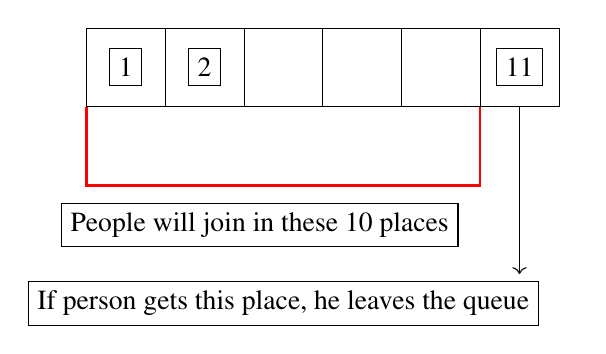
\begin{tikzpicture}
        \draw[step=1cm,black,very thin] (0,0) grid (6,1)  node[anchor=north west] {};
        \node[draw] at (0.5,0.5) {1};
        \node[draw] at (1.5,0.5) {2};
        \node[draw] at (5.5,0.5) {11};
        \node[draw] at (2.2,-1.5) {People will join in these 10 places};
        \draw[red,thick,solid] (0,0) -- (0,-1) -- (5,-1) -- (5,0);
        \node (A) at (5.5,0.0) {};
        \node (B) at (5.5,-2.25) {};
        \draw[->, to path={-| (\tikztotarget)}]
          (A) edge (B) ;
        \node[draw] at (2.5,-2.5) {If person gets this place, he leaves the queue};
        \end{tikzpicture}
    \caption{Queue}
    \label{fig:my_label}
\end{figure}
When a person comes, if $n=11$, then the person leaves without joining the queue.\\ So, $P_{11}$ is the probability of people leaving without joining the line.
\begin{align}
    P_{11}&=\rho^{11} P_{0}\\
    P_{11}&=1^{11} P_{0}\\
    P_{11}&= \frac{1}{11}
\end{align}
So, the probability that a person who comes and doesn't join the queue is $\frac{1}{11}$
\end{document}
